% ================= IF YOU HAVE QUESTIONS =======================
% Questions regarding the SIGS styles, SIGS policies and
% procedures, Conferences etc. should be sent to
% Adrienne Griscti (griscti@acm.org)
%
% Technical questions _only_ to
% Gerald Murray (murray@hq.acm.org)
% ===============================================================
%
% For tracking purposes - this is V1.9 - April 2009
\documentclass{sig-alternate}
  \pdfpagewidth=8.5truein
  \pdfpageheight=11truein
\usepackage{verbatim}
\usepackage{booktabs}
\usepackage{multirow}
\usepackage{graphicx}
\usepackage{epstopdf}

\begin{document}
% --- Author Metadata here ---
\conferenceinfo{SAC'15}{April 13-17, 2015, Salamanca, Spain.}
\CopyrightYear{2015}
\crdata{978-1-4503-3196-8/15/04...\$15.00.\\
http://dx.doi.org/10.1145/2695664.2695884
}  % Allows default copyright data (X-XXXXX-XX-X/XX/XX) to be over-ridden.
% --- End of Author Metadata ---
\title{Developers Assignment for Analyzing Pull Requests}
%\begin{comment}
\numberofauthors{3} 
\author{
% 1st. author
\alignauthor
Manoel Limeira de Lima J\'unior$\mathsf{^{1,2}}$ %\titlenote{Dr.~Trovato insisted his name be first.}
\\
       \affaddr{$\mathsf{^{1}}$Federal University of Acre}\\
      % \affaddr{1932 Wallamaloo Lane}\\
       \affaddr{Rio Branco $-$ AC, Brazil}\\
       \email{limeira@ufac.br}
% 2nd. author
\alignauthor Daric\'elio Moreira Soares$\mathsf{^{1,2}}$ \\
       \affaddr{$\mathsf{^{1}}$Federal University of Acre}\\
       \affaddr{Rio Branco $-$ AC, Brazil}\\
       \email{daricelio@ufac.br}
% 3rd. author
\alignauthor Alexandre Plastino$\mathsf{^{2}}$%\titlenote{The secretary disavows any knowledge of this author's actions.}
\\
       \affaddr{$\mathsf{^{2}}$Institute of Computing, Fluminense Federal University}\\
       \affaddr{Niter\'oi $-$ RJ, Brazil}\\
       %\affaddr{Dublin, Ohio 43017-6221}\\
       \email{plastino@ic.uff.br}
\and  % use '\and' if you need 'another row' of author names
%\begin{comment}
% 4th. author
\alignauthor Leonardo Murta$\mathsf{^{2}}$%\titlenote{This author is the
%one who did all the really hard work.}
\\
       \affaddr{$\mathsf{^{2}}$Institute of Computing, Fluminense Federal University}\\
       %\affaddr{1 Th{\o}rv{\"a}ld Circle}\\
       \affaddr{Niter\'oi $-$ RJ, Brazil}\\
       \email{leomurta@ic.uff.br}
}
%\end{comment}
\maketitle
\begin{abstract}
A new collaboration approach is becoming increasingly common in open-source projects: the pull request model. In this kind of collaboration, developers that do not belong to the core team of a project can submit contributions to the core team. In projects that receive many pull requests, the task of assigning developers to analyze them is a difficult one. In this work, we propose to use data mining techniques, more specifically, classification strategies, in order to suggest the most appropriate developers to analyze a contribution, considering the pull request model. The experiments were conducted using 21 open source projects, each one characterized by 14 attributes. The first set of experiments aimed at indicating just one developer to analyze the pull request. The obtained predictive accuracy ranged from 22.45\% to 68.27\%. The Random Forest classifier achieved the best result in 76\% on the projects. In the second set of experiments, we conclude that, when suggesting three developers to analyze a pull request, the chance of identifying the developer that actually analyzed the pull request ranged from 47.33\% to 95.47\%.
\end{abstract}
%A category with the (minimum) three required fields
\category{D.2.7}{Software Engineering}{Distribution, Maintenance, and Enhancement}[Version control]
%A category including the fourth, optional field follows...
\category{D.2.9}{Software Engineering}{Management}[Programming teams]
\terms{Management, Experimentation, Measurement}
\keywords{Pull-based development, pull request assignment, distributed software development}

\section{INTRODUCTION}
The usage of code hosting sites, such as GitHub, has increased significantly in the open source software development community \cite{briandoll_10_Million}. This growth has provided new opportunities for collaboration among developers, even if they do not belong to the core team of the project. In these cooperative environments, any developer can participate in a project by fixing bugs, or developing new features.

However, such collaborations would lead to a very uncontrolled software development environment. Aiming at enforcing control without restricting contributions to only the core team, a new collaboration approach has emerged: the pull request model. In this paradigm, a developer that does not belong to the core development team of a project can submit contributions to the project.

After receiving a pull request, a member of the core team needs to review it and take responsibility for either incorporating the contribution to the repository or not. The pull request can assume three states: merged, which means that the code has been incorporated; closed, representing that the request was not accepted; and open, indicating that the pull request has not yet been treated. If the changes are considered unsatisfactory, the developer from the core team in charge of analyzing the pull request can request changes or clarifications through comments. Therefore, requesters need to respond to comments and eventually update the pull request with new commits so that the pull request is re-evaluated ~\cite{gousios_ghtorent_2013}.

The decision to incorporate the pull request or not is one of the last stages of its life cycle \cite{gousios_ghtorent_2013, tsay_influence_2014}. Thus, a problem that precedes this step, and that gains importance in the process, is knowing which are the most suitable developers to evaluate and decide what action should be taken for each pull request.

Nowadays, 14\% of the projects in GitHub already adopt such collaboration model in dataset GHTorrent. In popular projects, which have an active community, a great number of pull requests is generated per month. On average, a single pull request takes 3.7 days to be analyzed. The analysis of a pull request can become a costly task for several reasons: the code can be extensive, changes made can affect multiple files, and the developer responsible for the analysis may be unaware of the features added by the pull request \cite{gousios_exploratory_2014}.

Although we could not find any other work on developers assignment for analyzing pull requests, this assignment problem is widely discussed in another context: processing of issues. Some studies recommend developers to analyze issues in open source projects \cite{anvik_automating_2006, anvik_reducing_2011}. This task, also known as triage, aims at finding the most appropriate developer to deal with a particular modification demanded by an issue. Time, knowledge, and workload of developers are some factors that, combined with the large number of issues, make this assignment process difficult and complex \cite{cavalcanti_challenges_2014}.

Pull requests differ from issues because they contain source code, providing information such as files added, changed, or removed, lines added and removed, and commits. Therefore, pull requests contain valuable information that can be extracted from the history of the version control repository.

In this paper we propose the use of classification algorithms over pull requests for ranking the most suitable developers to analyze them. Data classification is a process consisting of two steps: one of learning, and the other of classification. First, a classifier is built considering a training dataset. At this stage, the classification algorithm processes a set of already analyzed pull requests aiming at understanding which attributes influence the assignment of developers. After the construction of the classifier, it is possible to use it and to measure its accuracy, i.e., the percentage of tuples in the set of tests that were correctly classified \cite{han_data_2011}.

With the use of classification techniques, throughout 21 different projects, it was possible to obtain a prediction accuracy ranging from 22.45\% to 68.27\% in the task of identifying the developer that actually analyzed a pull request. In experiments in which three developers were indicated, the chance of identifying the developer that actually analyzed the pull request ranged from 47.33\% to 95.47\%.

This paper is organized as follows. Section 2 presents the database used in the experiments and the methodology. Section 3 contains the analysis of the obtained results. Section 4 discusses related studies and, finally, Section 5 provides conclusions and recommendations for future work.

\section{MATERIALS AND METHODS}
This section presents the projects and data attributes used in the experiments. Moreover, it also discusses the adopted methodology

\subsection{Projects}
This work uses a database that contains open ~source projects hosted by GitHub, extracted by the GHTorrent tool and exported to the database management system MySQL \cite{gousios_ghtorent_2013, han_data_2011}. This database contains 3,200,428 pull requests distributed in 8,510,504 projects, many of which use the methodology of contribution based on pull requests. Considering the projects that are not forks, 68 have more than 2,000 registered pull requests.

As we aim at assigning developers to pull requests, we use projects that received many pull requests and that have multiple developers to allocate them. If a project has five or less developers in the core team, a ranking of the three most suitable developers to analyze a pull request would be very close to the size of the team. 
%In this type of project, the use of a ranking generated by classification algorithms would be very similar to the actual distribution of pull requests on the team. 
Even with a large team, projects can adopt a policy where one or a few developers analyze pull requests. This kind of project is also out of the scope of our work.

Thus, four filters were established to select projects that are of interest in this study: i) projects with more than 2,000 pull requests; ii) projects with information about who analyzed the pull requests; iii) projects with many developers on the main team (with more than five members); and iv) projects where the majority class (MC) is not predominant (below 50\%), i.e., there is no single developer responsible for over half of the pull request analyses. 

After applying the filters over the 68 projects with 2,000 pull requests or more, it was observed that: 37\% (25 projects) had a predominating MC, 13\% (9 projects) had less than five developers in the team, and 19\% (13 projects) did not contain in the base GHTorrent information about which developers analyzed the pull requests. On the other hand, 31\% (21 projects) met the filters qualifications and were selected. Finally, pull requests that were analyzed by the requesters themselves were removed from the experiments. This decision aims at avoiding getting inconsistent results and simulating more closely the process of assigning the pull requests among the developers. 

Table 1 presents the characteristics of the selected projects: the size of the core team (developers who analyzed at least one pull request), the amount of pull requests analyzed in each project, and the average analysis time of pull requests merged (M) and closed (C) considering external requesters and the core team. It is worth to notice that some projects have less than 2,000 pull request due to our last filtering step, which removed pull requests analyzed by the same developer that filled the request in.
%\vspace{-0.2cm}
\begin{table}[htb]
\caption{Characteristics of the selected projects.}
\begin{tabular}{@{}l@{} p{0.1cm} @{}c@{} p{0.07cm} @{}c@{} p{0.07cm} @{}c@{} p{0.07cm} @{}c@{} p{0.07cm}@{}c@{} @{}l@{} @{}c@{}}
\hline
\multirow{3}{*}{\textbf{Project}} & \multirow{3}{*}{} & \multirow{3}{*}{\textbf{Team}} & \multirow{3}{*}{} & \multirow{3}{*}{\textbf{\begin{tabular}[c]{@{}c@{}}Pull\\ Request\end{tabular}}} &  & \multicolumn{7}{c}{\textbf{Average Time(days)}} \\ \cline{6-13} 
 &  &  &  &  &  & \multicolumn{3}{c}{\textbf{Core}} &  & \multicolumn{3}{c}{\textbf{External}} \\ \cline{6-13} 
 &  &  &  &  &  & \textbf{C} &  & \textbf{M} &  & \textbf{C} &  & \textbf{M} \\ \hline
akka             &  & 7   &  & 482   &  & 20.71 &  & 3.29  &  & 28.44 &  & 6.97  \\ 
angular          &  & 15  &  & 1,93  &  & 18.57 &  & 6.08  &  & 18.40 &  & 16.86 \\
Baystation12     &  & 14  &  & 2,364 &  & 1.71  &  & 0.45  &  & 2.93  &  & 0.61  \\
bitcoin          &  & 7   &  & 1,59  &  & 24.14 &  & 11.52 &  & 44.11 &  & 12.00 \\
brackets         &  & 27  &  & 2,745 &  & 15.98 &  & 3.28  &  & 26.36 &  & 9.19  \\
commcare-hq      &  & 11  &  & 2,468 &  & 1.26  &  & 0.78  &  & 1.54  &  & 1.18  \\
gaia             &  & 107 &  & 5,254 &  & 14.07 &  & 2.85  &  & 26.34 &  & 5.47  \\
infinispan       &  & 14  &  & 1,388 &  & 3.31  &  & 2.67  &  & 11.87 &  & 0.94  \\
ipython          &  & 11  &  & 1,83  &  & 9.93  &  & 6.28  &  & 34.02 &  & 9.91  \\
katello          &  & 20  &  & 877   &  & 16.67 &  & 0.93  &  & 8.41  &  & 7.87  \\
kuma             &  & 6   &  & 1,853 &  & 4.76  &  & 1.48  &  & 8.09  &  & 2.87  \\
metasploit       &  & 22  &  & 2,575 &  & 13.48 &  & 4.49  &  & 32.73 &  & 7.40  \\
pandas           &  & 10  &  & 958   &  & 17.29 &  & 5.19  &  & 35.29 &  & 9.15  \\
phobos           &  & 21  &  & 1,601 &  & 41.63 &  & 11.73 &  & 80.16 &  & 12.85 \\
puppet           &  & 45  &  & 1,497 &  & 25.35 &  & 4.63  &  & 51.36 &  & 13.09 \\
rails            &  & 29  &  & 7,403 &  & 22.55 &  & 3.53  &  & 46.78 &  & 9.02  \\
rosdistro        &  & 8   &  & 2,667 &  & 0.10  &  & 0.019 &  & 0.79  &  & 0.21  \\
scala            &  & 10  &  & 2,468 &  & 5.14  &  & 2.73  &  & 9.40  &  & 5.33  \\
-tg-station      &  & 9   &  & 1,054 &  & 3.23  &  & 2.97  &  & 8.92  &  & 3.87  \\
titanium\_mobile &  & 26  &  & 3,5   &  & 14.13 &  & 2.60  &  & 113.2 &  & 11.27 \\
xbmc             &  & 41  &  & 2,006 &  & 55.46 &  & 9.53  &  & 72.59 &  & 13.89 \\ \hline
\textbf{Average} &  & \textbf{21.90} &  & \textbf{2,401} &  & \textbf{15.69} &  & \textbf{4.14} &  & \textbf{31.51} &  & \textbf{7.62} \\ \hline
\end{tabular}
\end{table}

The average analysis time of pull requests was, approximately, 4 to 8 days when the pull request was merged (accepted) and 15 to 32 days when it was closed (rejected). It is worth highlighting that in some projects, such as Baystation12 and commcare-hq, the core team could analyze the external pull requests in up to three days on average. However, in other projects, such as rails, the time increases considerably, with average over 9 days when they are accepted and more than 46 days when they are rejected. In general, developers analyze the pull requests sent by requesters of the core team in less time than those sent by external requesters. The projects are written in a diverse range of programming languages, such as Scala, Python, Java, C, C++, Ruby, and JavaScript.

\subsection{Attributes}
The attributes used in the process of developer assignment, listed in Table \ref{tab:Table 2}, were extracted from the GHTorrent dataset based on works of bug triaging and also on semistructured interviews of Github developers \cite{gousios_exploratory_2014}. The target attribute of the problem (i.e., class) is the $15^{th}$ (final\_developer). The other attributes characterize the requester, the contribution, and the social interactions between the requester and the project. The attributes referring to lines of code (added and removed) and number of changed files were extracted directly from the repositories via the GitHub API. Attributes that were created or changed after the submission of the pull request, such as number of comments, were ignored, as they would not be available during submission.
\vspace{-0.4cm}
\begin{table}[htb]
\caption{Attributes of the projects.}\label{tab:Table 2}
\begin{tabular}{@{}c@{} p{0.1cm}@{} p{2.3cm} l@{} p{5.3cm}@{}}
\toprule
\textbf{Id} & \textbf{} & \textbf{Attribute} & \textbf{} & \textbf{Description} \\ \midrule
1 &  & watcher\_project &  & Indicates whether the project is one of the favorites of the collaborator. \\
2 &  & collaborator\_type &  & External collaborator or core team. \\
3 &  & commits\_pull &  & Amount of commits in a pull request. \\
4 &  & pull\_user &  & Amount of pull requests sent by the collaborator. \\
5 &  & pull\_merged\_user &  & Amount of pull requests accepted. \\
6 &  & pull\_closed\_user &  & Amount of pull requests rejected. \\
7 &  & ratio\_user\_merged &  & Rate of accepted pull requests. \\
8 &  & ratio\_user\_closed &  & Rate of rejected pull requests. \\
9 &  & followers\_user &  & Amount of collaborator's followers. \\
10 &  & follower &  & Amount of developers followed by the collaborator. \\
11 &  & follower\_project &  & Amount of developers in core team followed by the collaborator. \\
12 &  & lines\_additions &  & Amount of added lines of code. \\
13 &  & lines\_deletions &  & Amount of deleted lines of code. \\
14 &  & files\_changed &  & Amount of changed files. \\ 
15 &  & final\_developer &  & Who analyzed the pull request. \\ \bottomrule
\end{tabular}
\end{table}

\subsection{Methodology}
In order to identify the developer that actually analyzed a pull request, the following classification algorithms were used: i) Naive Bayes (NB), which is based on Bayes' theorem of calculate the probability of an instance to belong to each class \cite{han_data_2011, john_estimating_1995}; ii) J48, which uses the concept of decision tree and implements the C4.5 algorithm \cite{quinlan_c4.5:_1993}; iii) Random Forest (RF), which combines the predictions from different decision trees \cite{breiman_random_2001}; iv) IBk (Instance-Based), which is an implementation of k-NN (k-Nearest Neighbors), based on the idea of finding the nearest k neighbors of an instance and, thus, classify the new instance with the predominant class among neighbors \cite{aha_instance-based_1991, han_data_2011} and; v) the SMO (Sequential Minimal Optimization), which implements the SVM (Support Vector Machine) strategy and perform a nonlinear mapping to transform the training data into a higher dimension. Within this new dimension, it looks for a decisive boundary that separates the tuples of one class from another \cite{han_data_2011}. 

These algorithms belong to different paradigms of machine learning and are traditionally considered due to their competitive performance. Problems like the triage of issues also consider such algorithms \cite{lessmann_benchmarking_2008}.

We adopted the Weka\footnote[1]{http://www.cs.waikato.ac.nz/ml/weka/} tool during our experiments. It offers a wide collection of classification algorithms and provides the necessary support for the training and testing phases of the classification process. The following results were obtained from datasets with the attributes containing continuous values. Experiments were also performed after normalizing and discretizing the values, however, the accuracy obtained from the datasets with continuous attributes was better than with normalized or discretized attributes. 

With the aim of evaluating the input parameters of some algorithms, preliminary experiments were done, such as the variation of the value of k (number of neighbors) for IBk implementation and the variation of the SMO kernel. For IBk, the k values used were odd numbers from 1 to 15. For SMO, the following kernels were used: Polynomial, Puk, and RBF.

The evaluation was carried out using the 10-fold cross validation method. This strategy randomly divide the dataset into 10 partitions of the same size and the training and testing is performed 10 times. In each run, one of the ten partitions is used for testing and the rest for training \cite{han_data_2011}. We adopted the non-parametric Friedman test and the Nemenyi post-test \cite{pohlert_pairwise_2014} to identify statistically significant results \cite{demsar_statistical_2006}. In both statistical tests we adopted significance level of 0.05.

%In a second experiment, we propose a ranking of recommended developers for analyzing a pull request. We contrasted the proportion of recommendations that were able to identify the developer that actually analyzed the pull request with the majority class. Thus, it was possible to list the developers in ascending order, using the percentage of correct answers in cases where the algorithm indicated the developer that actually analyzed the issue in the first three positions of the ranking.

\section{RESULTS AND DISCUSSION}
Figure \ref{fig:smo} shows the boxplots of accuracy values obtained considering each kernel evaluated for the SMO algorithm, for all projects. 
%\vspace{-0.35cm}
\begin{figure}[htb]
\centering
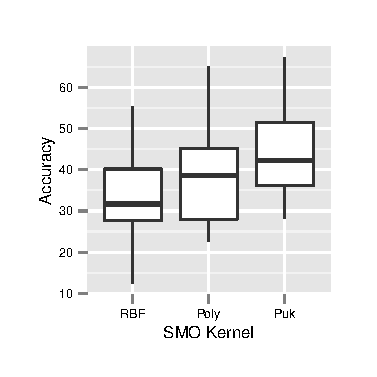
\epsfig{file=smo.eps}
\vspace{-0.4cm}
\caption{Accuracies of SMO.}\label{fig:smo}
\end{figure}

The top and bottom half boxes represent 50\% of the accuracies that are above or below the median (line that divides the chart), respectively; the remaining 50\% are represented by a vertical line. In this experiment, the Puk kernel achieved higher accuracies in all projects and was used in the next experiments. Using the Friedman test, the null hypothesis was rejected with p-value = 4.63e-09, indicating that there is a statistical difference between the results of the experiment. Using the Nemenyi post-test, we could observe that Puk kernel was statistically better than Poly (p-value = 0.0011) and RBF (p-value = 2e-09).

In the assessment of the input parameter k of the IBk algorithm, accuracy values for each value of k, ranging from 1 to 15, were obtained. Figure \ref{fig:ibk} shows boxplots of the accuracy values for the variations of k, ordered by the median values. Due to the p-value = 0.0175 of Friedman test, the statistical difference was also accepted. However, Nemenyi post-test showed no difference among the top variations. The variation with k = 5 was chosen as it obtained the best results in the ranking used to calculate the Friedman test.
%\vspace{-0.3cm}
\begin{figure}[h]
\centering
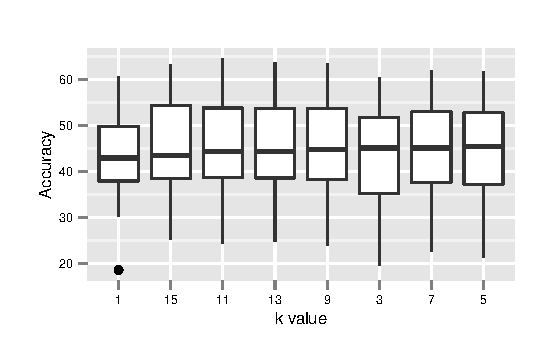
\epsfig{file=ibk.eps}
\vspace{-0.8cm}
\caption{Accuracies of IBk.}\label{fig:ibk}
\end{figure}

Due to these results, we adopted the Puk kernel for SMO and k = 5 for IBk in the further experiments.

\subsection{Accuracies of the Algorithms}
In the following experiments, the classification algorithms Naive Bayes (NB), J48, Random Forest (RF), IBk (k=5), and SMO (Puk) were evaluated. Table \ref{tab:Table 3} presents the accuracies obtained by these five algorithms over a continuous dataset for each of the 21 projects. The majority class (MC) column indicates the percentage of the predominant class of the dataset. This can be seen as a baseline, as always choosing the MC would lead to the informed accuracy. The best accuracies for each project are highlighted in bold. 

At first, the accuracies of projects titanium\_mobile, katello, and gaia, 60.71\%, 35.69\%, and 45.93\%, respectively, may seem low. However, the RF algorithm was able to improve the predominant class percentage by 236\% in titanium\_mobile (MC = 18.03\%), 187\% in katello project (MC = 12.43\%) and 103\% in gaia (MC = 22.59\%).

In the comparison among all classification algorithms, RF achieved the highest accuracies in 16 projects. For this experiment, the statistical difference is accepted once again with p-value = 2.63e-13 in the Friedman test. In the Nemenyi post-test, the RF algorithm obtained statistically better results compared to SMO (Puk) (p-value = 0.0006), J48 (p-value = 0.0003) and NB (p-value = 1.6e-13). We could not observe statistical difference between RF and IBk (k=5).
\begin{table}[t]
\vspace{-0.215cm}
\caption{Accuracies obtained for each project.}\label{tab:Table 3}
\begin{tabular}{@{}lc@{} p{0.12cm} @{}c@{} p{0.12cm} @{}c@{} p{0.12cm} @{}c@{} p{0.12cm} @{}c@{} p{0.12cm} @{}c@{}}
\toprule
\multirow{2}{*}{\textbf{Project}} & \multirow{2}{*}{\textbf{MC}} & \multicolumn{10}{c}{\textbf{Accuracy (\%)}} \\ \cmidrule(l){3-12} 
 &  &  & \textbf{NB} &  & \textbf{J48} &  & \textbf{RF} &  & \textbf{IBk} &  & \textbf{SMO} \\ \midrule
akka & 35.89 &  & 11.21 &  & 59.35 &  & \textbf{68.27} &  & 61.00 &  & 56.87 \\
angular & 33.68 &  & 8.86 &  & 34.20 &  & 40.21 &  & 36.58 &  & \textbf{42.90} \\
Baystation12 & 22.84 &  & 7.91 &  & 40.40 &  & 44.12 &  & \textbf{44.92} &  & 42.26 \\
bitcoin & 36.04 &  & 25.85 &  & 50.31 &  & \textbf{53.90} &  & 52.83 &  & 52.20 \\
brackets & 18.25 &  & 5.43 &  & 30.24 &  & \textbf{34.72} &  & 31.77 &  & 30.16 \\
commcare-hq & 40.36 &  & 14.87 &  & 50.37 &  & \textbf{52.43} &  & 51.34 &  & 51.46 \\
gaia & 22.59 &  & 9.69 &  & 43.87 &  & \textbf{45.93} &  & 45.41 &  & 34.53 \\
infinispan & 24.28 &  & 9.37 &  & 34.37 &  & \textbf{39.20} &  & 37.76 &  & 33.58 \\
ipython & 29.90 &  & 8.49 &  & 45.79 &  & 48.98 &  & \textbf{49.32} &  & 48.05 \\
katello & 12.43 &  & 10.03 &  & 34.31 &  & 35.69 &  & \textbf{36.03} &  & 31.02 \\
kuma & 43.66 &  & 19.43 &  & 59.47 &  & \textbf{61.74} &  & 61.31 &  & 56.72 \\
metasploit & 40.27 &  & 5.09 &  & 49.55 &  & \textbf{52.62} &  & 48.51 &  & 51.34 \\
pandas & 42.69 &  & 17.96 &  & 63.37 &  & \textbf{67.44} &  & 61.80 &  & 67.12 \\
phobos & 31.71 &  & 4.31 &  & 33.58 &  & \textbf{39.58} &  & 37.21 &  & 36.14 \\
puppet & 20.44 &  & 4.68 &  & 35.87 &  & \textbf{41.95} &  & 35.74 &  & 33.07 \\
rails & 22.96 &  & 16.34 &  & 18.03 &  & 22.45 &  & 21.25 &  & \textbf{27.27} \\
rosdistro & 28.16 &  & 13.57 &  & 45.82 &  & \textbf{50.32} &  & 47.02 &  & 39.59 \\ 
scala & 33.50 &  & 10.77 &  & 56.09 &  & \textbf{60.14} &  & 57.39 &  & 51.15 \\
-tg-station & 37.86 &  & 4.56 &  & 39.09 &  & \textbf{44.22} &  & 43.36 &  & 40.71 \\
titanium\_mobile & 18.03 &  & 12.51 &  & 57.89 &  & \textbf{60.71} &  & 57.60 &  & 46.00 \\
xbmc & 24.93 &  & 11.57 &  & 36.40 &  & \textbf{39.44} &  & 37.79 &  & 33.70 \\ \midrule
\textbf{Average} & \textbf{29.55} & \textbf{} & \textbf{11.07} & \textbf{} & \textbf{43.73} & \textbf{} & \textbf{47.81} & \textbf{} & \textbf{45.52} & \textbf{} & \textbf{43.14} \\ \bottomrule
\end{tabular}
\end{table}
\vspace{-0.315cm}

The same experiments performed using the datasets with continuous attributes were repeated for the dataset with normalized and discretized attributes. Figure \ref{fig:dc} shows boxplots, sorted by the median, with the accuracies of all algorithms considering the continuous (C) and discrete (D) datasets. 
The Random Forest algorithm using continuous bases $ – $ RF(C) $ - $ achieved the best accuracy in 16 of the 21 projects. The second best algorithm was IBk with k = 5, also using the continuous dataset $ - $ IBk(C) $ - $ achieving the best accuracy in three projects and the second best result in 11 projects. 
%\vspace{-0.3cm}
\begin{figure}[h]
\centering
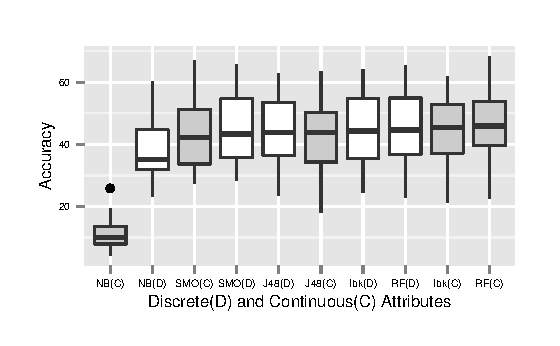
\epsfig{file=dc.eps}\label{fig:dc}
\vspace{-0.8cm}
\caption{Accuracies with continuous and discrete attributes.}
\end{figure}

Thus, we can conclude that in 76\% of the projects the best strategy was the RF(C), reaching an average accuracy of 47.81\%. The titanium\_mobile project achieved the biggest improvement between the MC and the RF(C): 236\%. Considering the differences between the accuracy of RF(C) and the MC, we could not observe improvements only in the rails project. It is important to highlight that the average gain of RF(C) in relation to the MC was 61\%.
\begin{figure*}
\centering
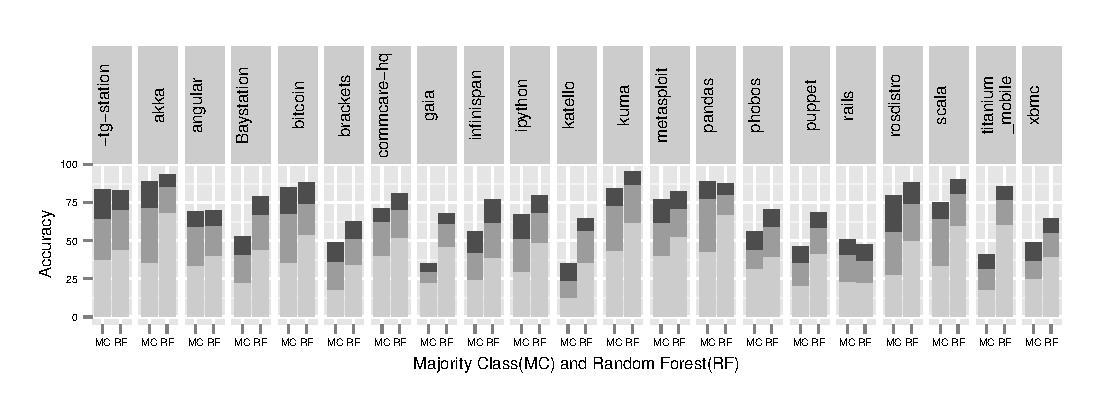
\epsfig{file=rank.eps}
\vspace{-0.8cm}
\caption{Ranking for assignment of developers.}\label{fig:rank}
\end{figure*}
\vspace{1cm}
\subsection{Ranking of developers}
We recognized that sometimes the first recommendation of a developer to analyze a pull request might not work, as the recommended developer may be unavailable for some reason. Aiming at mitigating this problem, we also evaluated the accuracy of recommending a rank of three developers for analyzing each pull request. In this experiment, the chance of identifying the developer that actually analyzed the pull request ranged from 47.33\% to 95.47\%.

Figure \ref{fig:rank} shows the percentage of the three majority classes in the project (MC bars), i.e., the three developers who analyzed the most pull requests. It also present the percentage of success for the first three recommendations made by the Random Forest classifier using the continuous datasets (RF bars). Each color tone in the bars corresponds to the percentage of accuracy provided by each recommendation when the developer that in fact analyzed the pull request had been recommended. 
%It is worth noticing that our baseline is still only the first MC (lighter bar), as it would not be possible to correctly combine the three MC recommendations. 
However, in the following discussion we use the combined MC bar as a theoretical limit.

The results of the ranking of developers recommended for analyzing pull requests can be divided into four groups: i) projects in which the ranking would be an option to decrease the error rate in assignments. This usually applies for projects with relatively small teams: less than 15 developers (-tg-station, akka, angular, bitcoin, pandas, and rosdistro); ii) projects where the ranking improves the recommendation, but cannot reach a significant gain than that of the three MC combined (brackets, commcare-hq, infinispan, ipython, kuma, phobos, scala, and xbmc); iii) projects with many developers in which the ranking reveals a promising strategy, significantly improving the success rate in the indication of three developers even if compared to the three MC combined: the puppet project is improved by 48\%, the titanium\_mobile project is improved by 109\%, the Baystation12 project is improved by 50\%, the katello project is improved by 83\%, and the gaia project is improved by 100\%; and iv) projects that even with many developers and without a predominant MC failed to present good results when considering the three MC combined (rails, metasploit). However, when considering only the first MC, which is a natural baseline, their results when adopting a rank of recommendations become relevant.

It is important to highlight that some projects have a high accuracy when three developers are suggested. For example, the kuma project presented accuracy of 95.47\%. In this case, the majority class considering the top three developers is also high: 84.56\%. However, when observing the recommendation error instead of the recommendation accuracy, it is possible to note that our approach would miss (i.e., not suggest the correct developer out of the three suggestions) in only 4.53\% of cases. Conversely, when considering the combination of the three MC, the error rate is 15.44\%. Thus, even for this case, the proposed approach shows a significant reduction of errors of 70\%.

\section{RELATED WORK}
Few studies have analyzed the influence of socio-technical factors on the decision to accept (merge) a pull request or not. Gousios et al.~\cite{gousios_exploratory_2014} sought to understand the life cycle of pull requests to evaluate the factors that contribute to their acceptance. The experiments were performed on 291 projects and 166,884 pull requests extracted by GHTorrent. The projects had standardized test code, allowing the study of how such attribute influence in the merge of pull requests.

The authors concluded that the presence of test code does not affect the time or the decision of accepting pull requests. They also claim that there is no special treatment for pull requests from developers of the core team. With the results, the authors infer that the decision to accept is strongly and positively influenced by the fact that the pull request modifies a code that was recently changed in the repository. Finally, they suggest that the acceptance time is inversely proportional to the merge load of the requester, in other words, the higher the percentage of pull requests accepted, the lesser the time it takes the pull request to be analyzed~\cite{gousios_exploratory_2014}.

Tsay et al.~\cite{tsay_influence_2014} held an analysis of the association of socio-technical measures with the probability of accepting pull requests in open source development project. Data from 12,482 projects and 659,501 pull requests were extracted from GitHub using Google BigQuery.

The study proposed a statistical model that associate socio-technical measurements with the probability of the pull request being accepted. It concludes that pull requests with many comments decrease the likelihood of acceptance by 54.6\%. However, the presence of the test code and some social factors improves the likelihood of merge \cite{tsay_influence_2014}. 
Regarding social factors, the study reveals that if the requester follows a developer of the core team, the probability of acceptance increases by 187\%. The greater the number of interactions between the requester and the project before sending the pull request, such as the participation in issues, pull requests, and comments on the project, the higher the likelihood (35.6\%). In addition, requesters with many followers increase the chances by 18.1\% \cite{tsay_influence_2014}.

These related works focus on classifying and exploring the reasons that influence the acceptance of pull requests. Our work focuses on a different problem in the life cycle of a pull request, prior to the analysis made by the presented studies: who should analyze the pull request?

In a work similar to ours, Yue et al.~\cite{yu_reviewer_2014} used the Vector Space Model technique to measure the similarity of a new pull request with the existing ones. Furthermore, they consider the comments to determine the score of the indicated developers to review the pull request. To evaluate the performance of their approach, they used a database with 10 open source projects and measured precision and recall of the recommendations.

Our approach contributes by suggesting a ranking of developers who, according to the history of the repository, would be the most suitable for analyzing a new pull request. Differently from Yue et al.~\cite{yu_reviewer_2014}, our work does not use information that arise during the life cycle of the pull request, which is not available during the pull request submission. Furthermore, we use the accuracy of the classification algorithms to measure our performance.

\section{CONCLUSIONS}

In this work, different classification algorithms were evaluated for the task of forecasting the developers that should be responsible for the analysis of a pull request. The strategy with the best accuracy in 76\% of the projects was the Random Forest algorithm using datasets with continuous attributes. This algorithm achieved, on average, 47.81\% of accuracy. When observing the difference between the obtained accuracy and the majority class, the gain was 61\%, on average.

The experiments also considered the recommendation of three developers in a ranking, rather than just one developer. The accuracy when three developers are recommended was significantly increased in projects such as titanium\_mobile, Baystation12, katello, and gaia, where the distribution of pull requests for analysis is not concentrated in a single developer. In projects where the pull requests are analyzed by fewer developers, our approach can be used as an alternative to minimize the error of assign wrong developers. The approach did not produce good results for projects with a predominant majority class as well as the rails and metasploit project, despite having many developers on their teams. 

Finally, in future work we intend to investigate new predictive attributes in different granularities, such as source code content. This aims at finding the best characteristics to determine the developers that should analyze each pull requests. The addition of new attributes, together with the use of attribute selection strategies and a preprocessing step might improve the accuracies of our approach.

\section{Acknowledgments}
We would like to thank FAPERJ, CNPq and CAPES for the financial support.
%\vspace{-0.28cm}
\bibliographystyle{abbrv}
\bibliography{MyBibLatex}
\end{document}
